\subsubsection{Average Transmission Time}
	When the network is saturated, it becomes clear that scenarios without any knowledge processing capabilities are unable to prioritise what is sent and all observations experience a uniform time, shown in Figure \ref{fig:sim:res:sat:variable:delmean}, but scenarios, such as HK-HK-HK, MK-HK-NK or MK-MK-NK are able to prioritise.
	\begin{figure}[H]
	\centering
	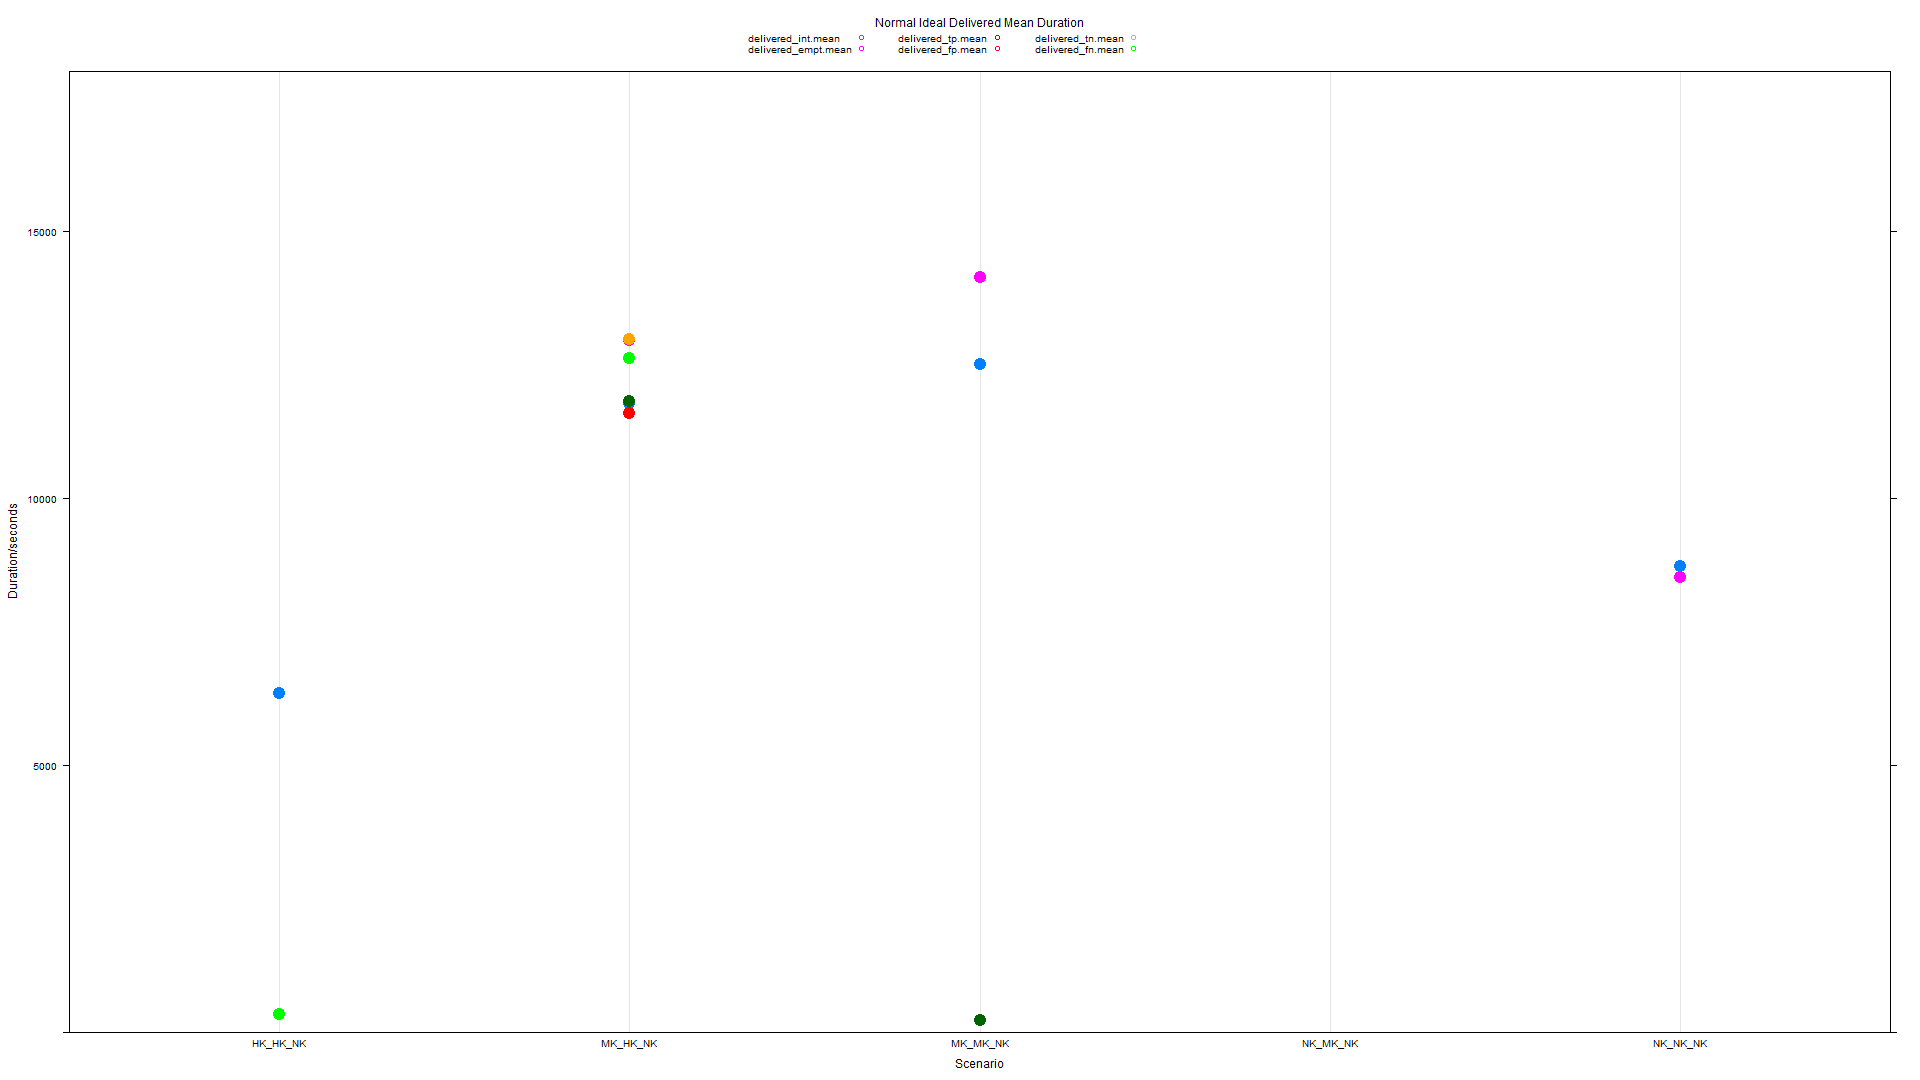
\includegraphics[width=\textwidth]{Chap7/figures/plots/normal_ideal/delivered_mean.png}
	\caption{Delivered Observations Mean Transmission Time for Normal Saturation and Ideal Transmission Rate}
	\label{fig:sim:res:norm:ideal:delmean}
	\end{figure}






\subsubsection{Delivered vs. Undelivered}
	Figure \ref{fig:sim:res:norm:ideal:delundel} shows that, when the network is not saturated and the transmission rate remains at the maximum, almost all observations are received by the DA node, regardless of the scenario. 







\subsubsection{Interesting vs. Empty}
	The pattern of interesting vs empty observations is clearest when looking at a saturated network. Figures \ref{fig:sim:res:sat:ideal:emptint} and \ref{fig:sim:res:sat:variable:emptint} show that, of the total observations delivered, HK-HK-HK has the most interesting observations. When the transmission rate is ideal, HK-HK-HK is still ahead but MK-HK-NK is slightly less than the central processing scenarios, in terms of interesting observations. Comparing this with the mean transmission time (Figure \ref{fig:sim:res:sat:ideal:delmean}), MK-HK-NK has a lower transmission time for interesting observations, while still delivering a similar amount.

	Under normal saturation (Figures \ref{fig:sim:res:norm:ideal:emptint}\ref{fig:sim:res:norm:variable:emptint}), the split is fairly uniform. 





\subsubsection{True Positive vs. False Positive}







\subsubsection{True Negative vs. False Negative}
	
	\begin{figure}[H]
	\centering
	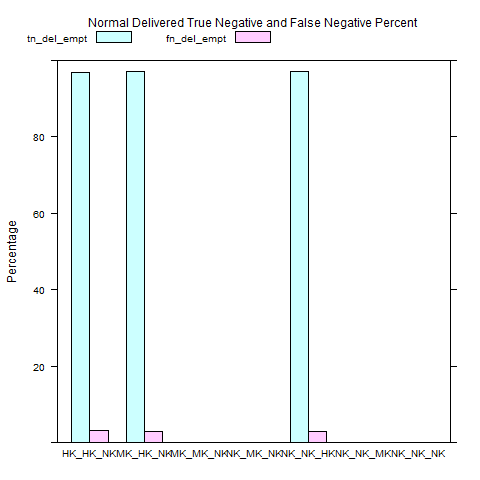
\includegraphics[width=\textwidth]{Chap7/figures/plots/normal_ideal/tnvsfn_percent.png}
	\caption{TN vs FN Observations for Normal Saturation and Ideal Transmission Rate}
	\label{fig:sim:res:norm:ideal:tnfn}
	\end{figure}

	\begin{figure}[H]
	\centering
	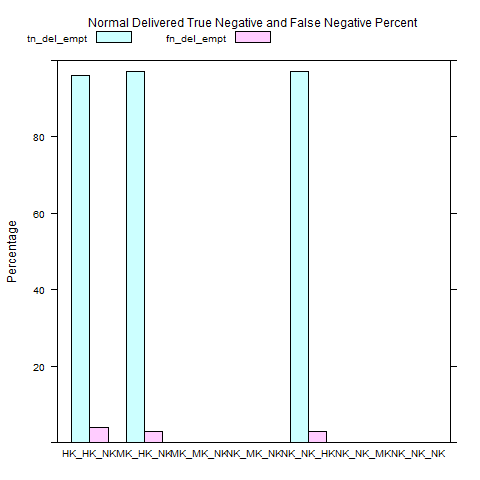
\includegraphics[width=\textwidth]{Chap7/figures/plots/normal_variable/tnvsfn_percent.png}
	\caption{TN vs FN Observations for Normal Saturation and Variable Transmission Rate}
	\label{fig:sim:res:norm:variable:tnfn}
	\end{figure}

	\begin{figure}[H]
	\centering
	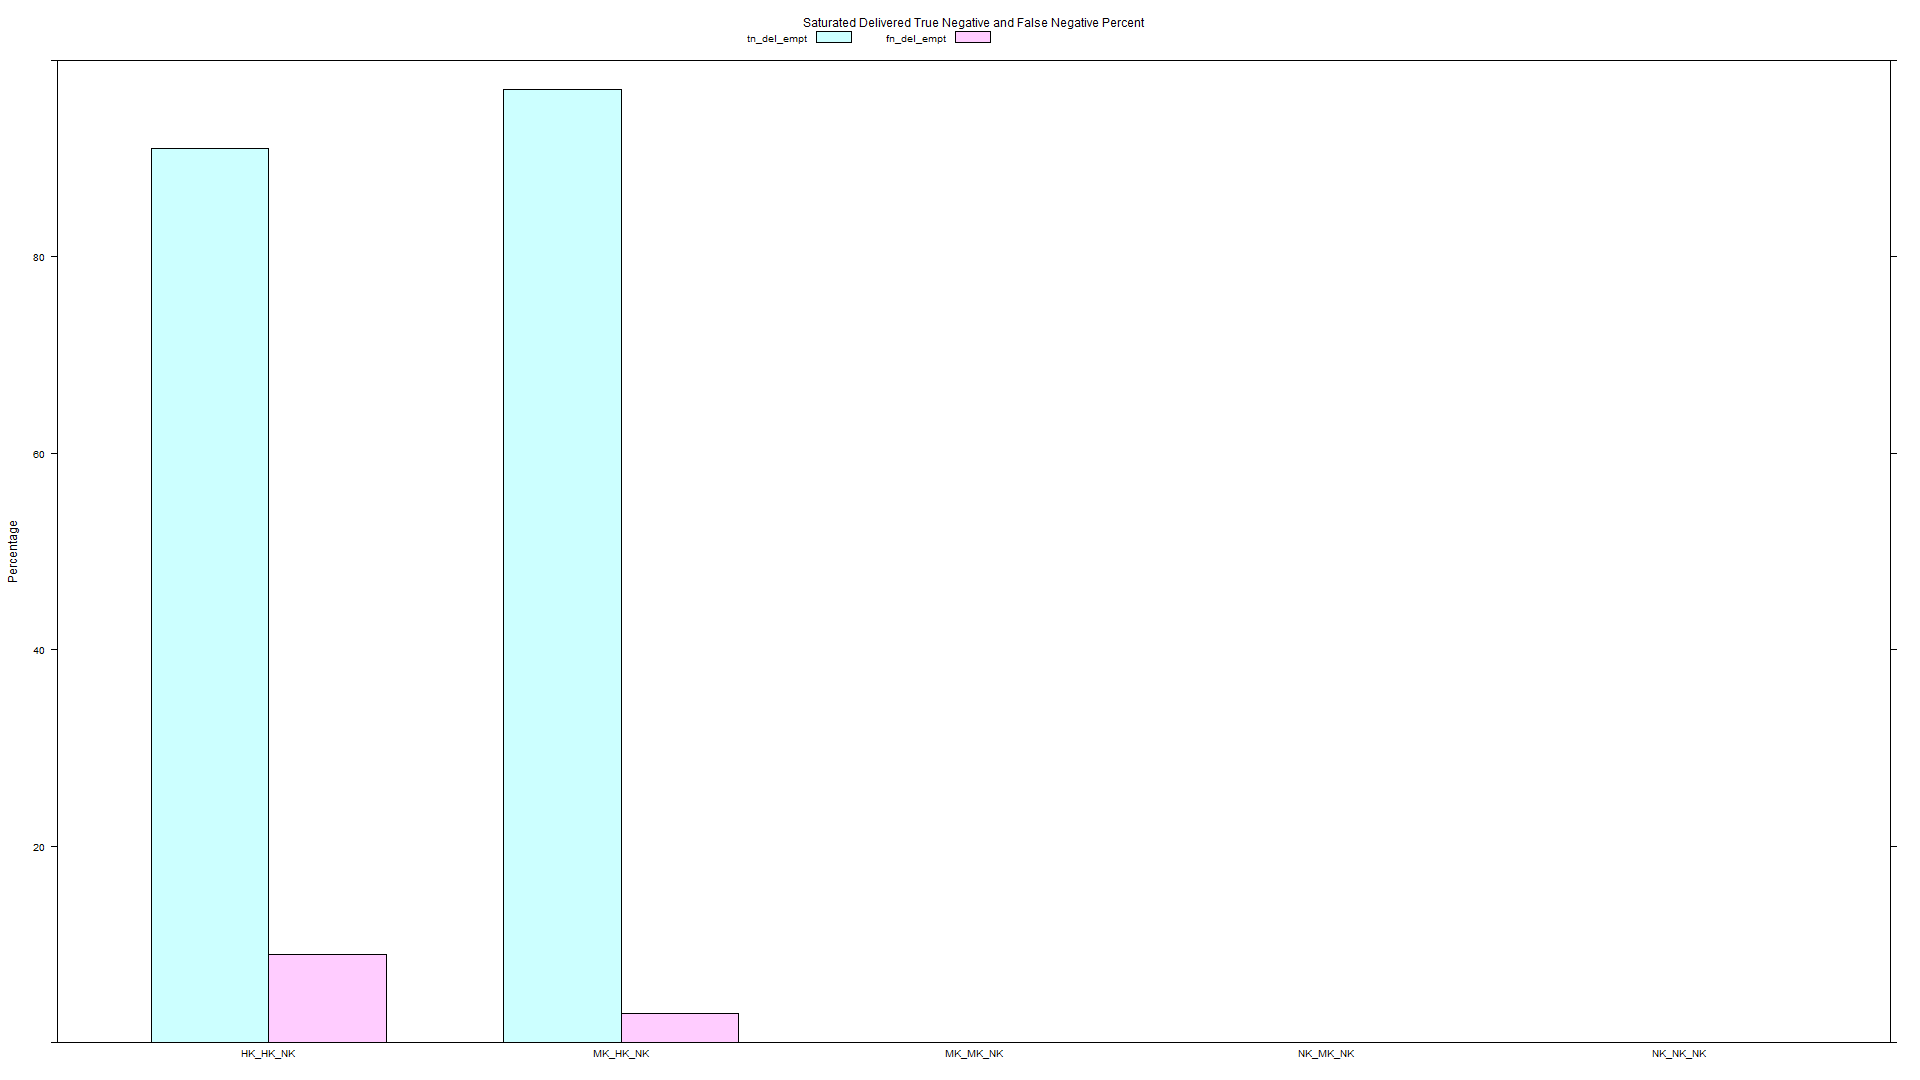
\includegraphics[width=\textwidth]{Chap7/figures/plots/saturated_ideal/tnvsfn_percent.png}
	\caption{TN vs FN Observations for Saturated Saturation and Ideal Transmission Rate}
	\label{fig:sim:res:sat:ideal:tnfn}
	\end{figure}

	\begin{figure}[H]
	\centering
	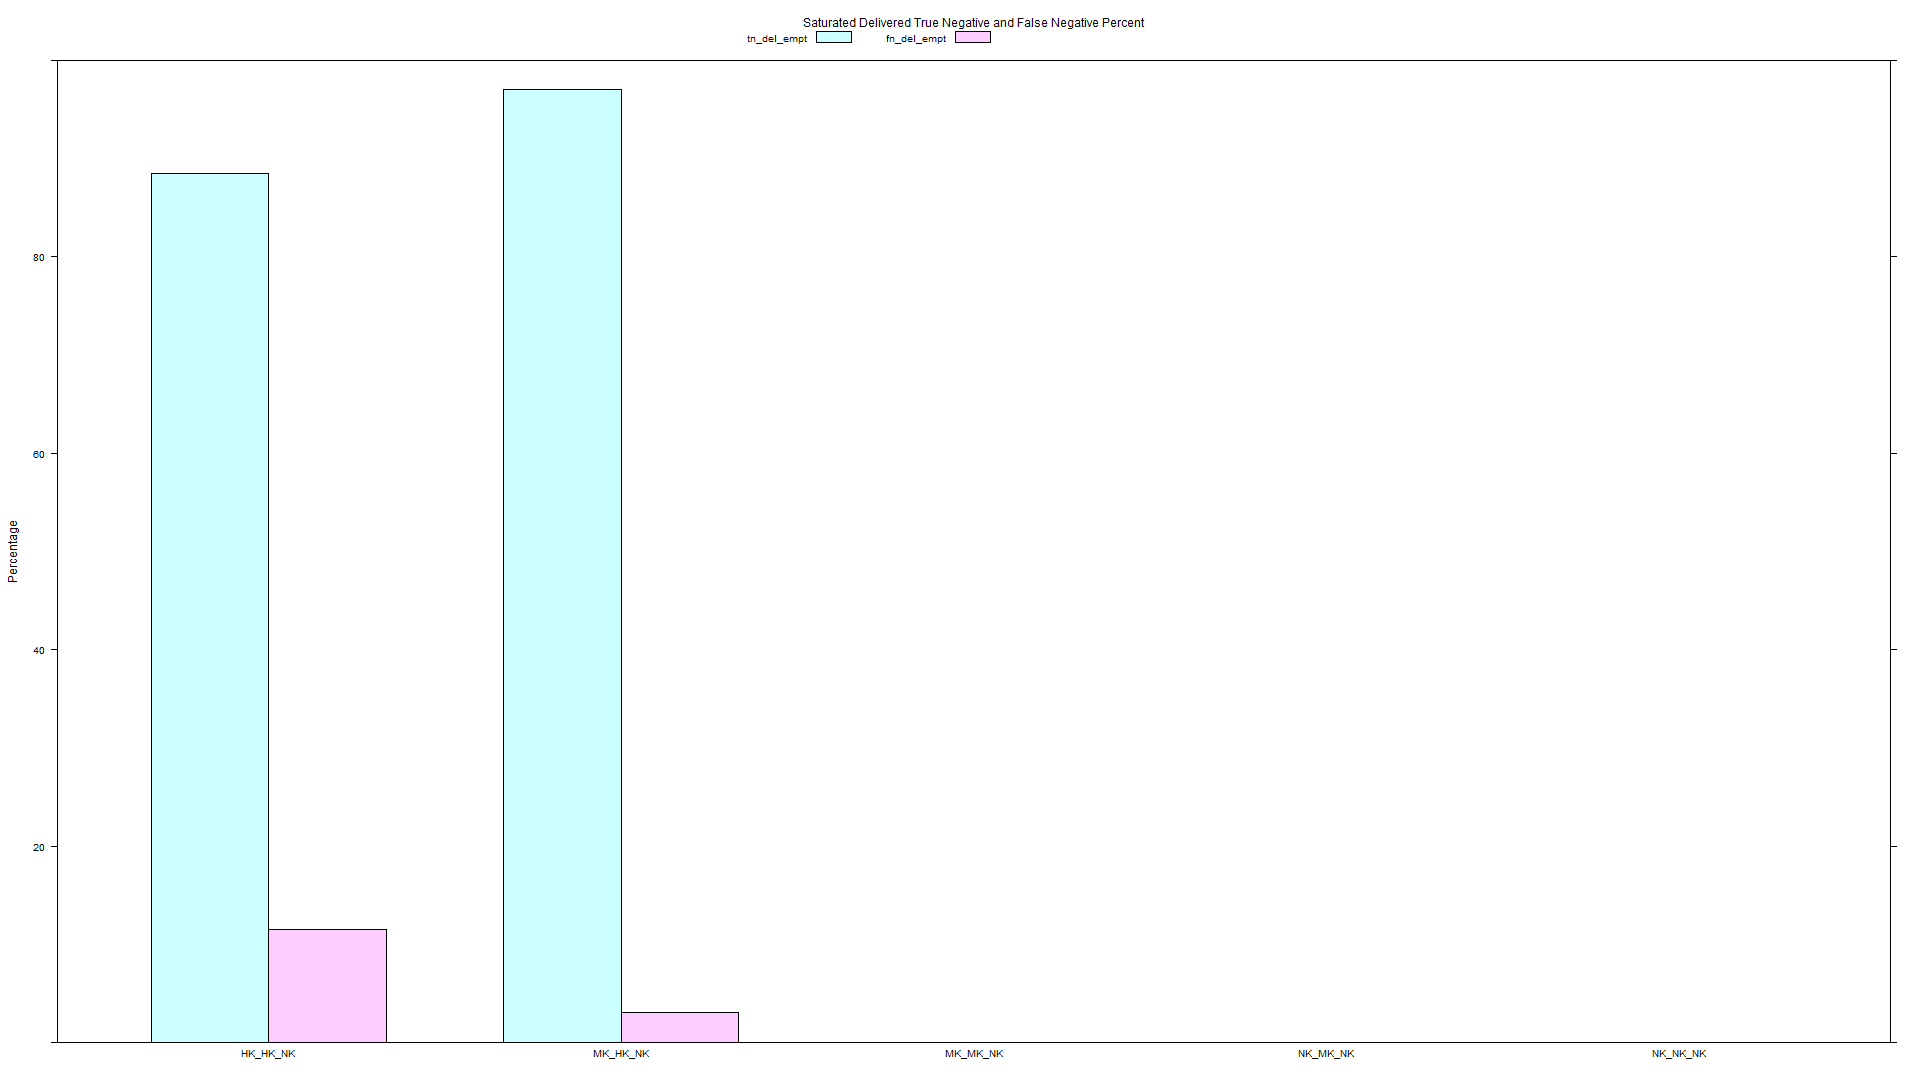
\includegraphics[width=\textwidth]{Chap7/figures/plots/saturated_variable/tnvsfn_percent.png}
	\caption{TN vs FN Observations for Saturated Saturation and Variable Transmission Rate}
	\label{fig:sim:res:sat:variable:tnfn}
	\end{figure}